%%=============================================================================
%% Model
%%=============================================================================

\chapter{\IfLanguageName{dutch}{Model}{Model}}
\label{ch:model}



\section{Inleiding}

In dit hoofdstuk behandelen we de elementen die impact ondervinden van een architectuur verandering, specifiek de transformatie van een monolithische architectuur naar microservices.

De elementen verdelen we op in twee categorieën. De eerste categorie bevat alle aspecten die te maken hebben met het financiële plaatje. Hieronder zullen elementen zoals ontwikkelingstijd, loonkost, investeringen in een nieuwe infrastructuur, … . \\
De tweede categorie zal alles bevatten die onderdeel uitmaakt van de sociale impact. Denk hier bij over de impact op het personeel. Een bedrijf die al 20 jaar hetzelfde systeem gebruikt, zal mensen te werk stellen die het moeilijk zullen hebben met grote veranderingen.

Het is bijna onmogelijk om een correct model op te stellen die voor elke bedrijfssituatie zal werken. Het doel van dit model is om alle elementen aan te halen waarbij een bedrijf eventueel rekening zal moeten houden. Bij elk element wordt er een voorbeeld gegeven die vertrekt vanuit een fictionele bedrijfssituatie die vermeld wordt in het begin van het hoofdstuk.

\section{Het financiële apsect}

De kosten die een bedrijf zal maken om te transformeren van een monolithische architectuur naar een systeem bestaande uit microservices zal voor ieder bedrijf anders zijn. Voor dit onderzoek en voor het opstellen van ons model, vertrekken we altijd uit het standpunt van een bedrijf met 50 programmeurs die al 5 jaar werkt met een monoliet. 

\subsection{Loonkost}

In vele gevallen zal de loonkost de grootste kost zijn voor een bedrijf. Volgens \emph{https://loonkost.besox.be/} kost de gemiddelde developer met een maandelijkse bruto loon van 3500 euro, 5160.72 euro per maand of 61.928.63 euro per jaar.

Hoeveel personen je nodig hebt om de transformatie uit te voeren hangt natuurlijk af van de grootte van het systeem en de manier waarop het bedrijf met zijn \emph{resources} om springt. 
Als het aantal benodigde werkkrachten is vastgelegd, komt het bedrijf op een volgend kruispunt te staan over hoe ze deze plaatsen zullen invullen.\\ Een eerst optie is om de werkkrachten te halen uit het bestaande personeel. In sommige gevallen zal dit niet mogelijk zijn omdat de nodige kennis niet aanwezig is of om dat het huidige systeem die nodig is om het geld in het laadje te brengen, onderhouden moet worden. De tweede optie is om extra personeel aan te werven, hetzij consultants of vaste werknemers.\\ 
Als ervoor consultants gekozen wordt, heb je het voordeel dat de kosten afgeschreven kunnen worden op het project. Wanneer het project klaar is, kan het bedrijf zich makkelijk ontdoen van de tijdelijke werkkrachten.  Het grootte nadeel is dat de kennis van de nieuwe architectuur grotendeels verloren gaat. Dit is een onrechtstreekse kost die moeilijk in kaart te brengen is en veel bedrijven zullen hier geen rekening mee houden. Maar op lange termijn kan deze ontbrekende kennis voor onvoorziene kosten zorgen. Het beste scenario is wanneer je de twee opties kan combineren. Het bestaande personeel krijgt de optie om door te groeien en consultants kunnen het \emph{legacy} werk tijdelijk overnemen.

\subsection{Tijd}

De uitspraak \emph{time is money} is ook hiervan toepassing. Hoe langer de transformatie duurt, hoe sneller de kosten oplopen. Er zal ook grotere kans zijn op onvoorziene kosten.\\
In vele gevallen zal de bestaande monoliet ook niet geüpdatet worden en enkel onderhouden worden. Onderhoud is een kost die niet afgeschreven kan worden, bedrijven willen dit dus zo veel mogelijk vermijden. Mits het huidige systeem ook geen updates krijgt, wordt er ook geen extra meerwaarde gecreëerd voor het bedrijf.

\subsection{Infrastructuur}

De kosten voor infrastructuur zijn ook per bedrijf verschillend. Voor de simpelste microservice te maken in AWS heb je enkel een \emph{lambda} en een \emph{API gateway} nodig. Deze miscroservice is heel beperkt in functionaliteit en in sommige gevallen heb je ook nog andere infrastructuur nodige zoals een EC2 server en een eventuele database. AWS factureert per aantal API calls, zie figuur \ref{awscost}.

\begin{figure}[!htb]
     \centering
    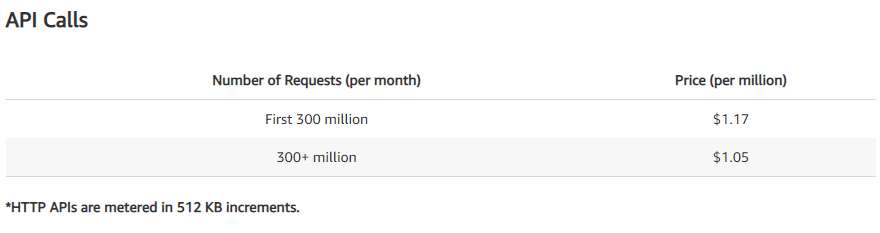
\includegraphics[width=13cm,height=13cm, keepaspectratio]{AWScosts.png}    
    \caption{kosten voor het gebruik van een standaard AWS api gateway \label{awscost}}
\end{figure}

Hieronder valt ook de veranderingen van technologieën.

\section{Het sociale aspect}

In dit hoofdstuk worden de effecten of veranderingen die aan de transformatie verbonden zijn besproken. Deze effecten kunnen zowel positief als negatief zijn, bedoeld of onbedoeld, direct of indirect.

\subsection{Personeel}

De transformatie van een monoliet naar microservices kan een impact hebben op de dagelijkse activiteiten. Tijdens de transformatie kan er gekozen worden voor een nieuwe technologie en kan de systeem infrastructuur aanpassen. Uit het onderzoek van ~\autocite{Schaik2014} blijkt dat er meer weerstand is op complexe veranderingen.  

Hoe duidelijker de verandering is, hoe minder weerstand er zal geboden worden tegen deze verandering.

Omscholing zal ook geld en tijd kosten. Sommige bedrijven willen investeren in hun personeel en bieden hen de kans aan om kennis op te doen over de nieuwe technologie. Deze investering garandeert geen succes.

Verandering zal niet altijd iedereen kunnen overtuigen. De idealen van personen kunnen niet meer in dezelfde lijn liggen als die van het bedrijf. In sommige gevallen kan dit leiden tot een scheiding tussen de twee partijen.

\subsection{Activiteiten}

Tijdens en vooral na de transformatie, zullen de dagelijkse activiteiten van het personeel er anders uit zien. Teams kunnen onderverdeeld worden in kleinere teams die verantwoordelijk zijn voor één of meerdere microservices. Er kunnen nieuwe functies of rollen ontstaan, maar ook bestaande functies kunnen verdwijnen.  

\section{Overzicht}

De overgang van een monolithische architectuur naar microservices zorgt voor vele uitdagingen. Het bedrijf zal een goede schatting moeten maken van de financiële kosten. Een dergelijke transformatie creëert op korte termijn weinig bedrijfswaarde. De kosten zullen stijgen waarbij de winsten op korte termijn niet direct omhoog zullen gaan. Aandeelhouders kunnen daarom niet altijd overtuigd worden om een dergelijke verandering uit te voeren.

Het opgemaakte model bestaat uit vijf pijlers
\begin{itemize}
    \item Tijd
    \item loonkost
    \item infrastructuur
    \item personeel
    \item activiteiten
\end{itemize}

Een bedrijf kan deze vijf pijlers als basis gebruiken om in te schatten wat de mogelijke impact zal zijn van de transformatie.

